\subsection{Exercício 10}

Observamos pelo exercício anterior são a árvore de regressão e os K-vizinhos-mais-próximos. Contudo, iremos comprovar estatisticamente através dos testes: t.test e wilcox

Após obtermos os dois melhores modelos, pretendemos verificar se são estatisticamente significativos e para isso recorremos a um \textbf{t.test} e um \textbf{wilcox.test}. Utilizando um nível de significância de 5\% e analisando o p-value obtido em cada um dos testes, concluímos que não existe uma diferença significativa entre os dois melhores modelos para ambos os testes.

\begin{table}[h!]
	\caption{Tabela com valores p-value para o t.test e wilcox.test}
    \begin{center}
    \begin{tabular}{|c|c|c|}
    \hline
    & \textbf{p-value} \\
    \hline
    t.test & 0.5255\\
    \hline
    wilcox.test & 0.5966\\
    \hline
    \end{tabular}
    \label{tab:my_label}
    \end{center}
\end{table}

Concluímos que a árvore de regressão e os K-vizinhos-mais-próximos são significativamente iguais. Para isso, utlizamos um boxplot e verificamos que a técnica da árvore de decisão tem, ligeiramente, um melhor desempenho como se pode ver na Fig 11.

\begin{figure}[htbp]
\centerline{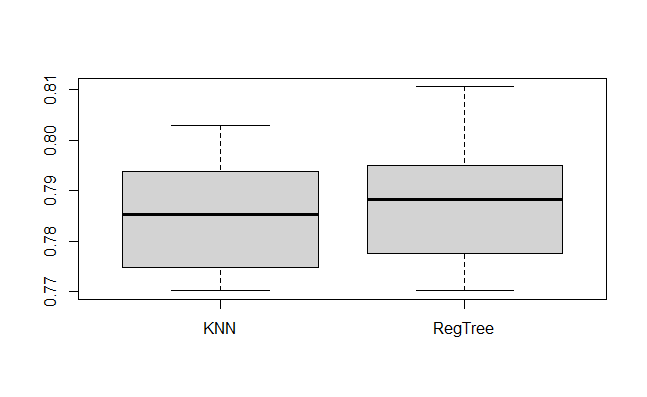
\includegraphics[width=9.5cm]{images/ex10_boxplot.png}}
\caption{Boxplot com o desempenho da técnica KNN e Árvore de Regressão}
\label{ex10_boxplot}
\end{figure}
